\chapter{Literature Study and Theoretical Framework}
\label{ch:literature}
%Overview of Manufacturing, MAS and framework.
The manufacturing industry is and will be one of the wealth generators of the world economy. A shift towards a modular production process, called the fourth industrial revolution, results in a demand for products with high quality at lower cost while being highly customized. This results in new ways of controlling the production. High-performing computing, the internet, universal access and connectivity, and enterprise integration all contribute. Overall the consensus is that only the companies that fully leverage the information, its availability, the ability to exchange it seamlessly and to process it quickly, are the companies that can meet the high demand of the consumers \citep{monostori2006agent}.

The so-called agent-based computation is a solution for many of the problems that arise from this new trend. By having autonomous agents, who can address changes adaptively and are distributed in nature, intelligent solutions are available \citep{monostori2006agent}.

In this literature review, an overview of the manufacturing processes and current agent technologies/solutions is given. Using such a decentralized agent solution is only optimal when certain process and design requirements are realised on the manufacturing side. We will derive a framework  on the basis of which one can decide between a centralized or decentralized system. After the framework is explained, we will give an overview of negotiation solutions in agent systems. From this we find a new approach to design a multi-agent system for a business process.

\section{Manufacturing Processes}

A new paradigm shift in the discrete manufacturing world requires a production that is competitive but also sustainable. Most of these solutions lie in the field of Cyber-Physical systems. A Cyber-Physical entity is one that integrates its hardware with a cyber-representation as a virtual representation. By doing so, it combines two worlds: the embedded systems and the software worlds. By doing so it breaks the traditional automation pyramid and introduces a new more decentralized way of function \citep{leitao2016smart}. This is visualized in \Cref{fig:traditional-automation-pyramid1}. %By making these systems intelligent, and connecting the design principles, the current lacking of industrial can be fully leveraged.
	
\begin{figure}[h]
\centering
\includegraphics[width=0.9\linewidth]{"img/traditional automation pyramid1"}
\caption{The breaking of the traditional automation pyramid (left) and the future of a new more decentralized way of function (right). Image from \citep{monostori2016cyber}.}
\label{fig:traditional-automation-pyramid1}
\end{figure}

The traditional automation pyramid is very similar to the multiple layers in the manufacturing process, which have been standardised by the American National Standards Institute (ANSI) \citep{harjunkoski2009integration}. The integration of the planning and control in the manufacturing process has many aspects. Below a short overview of manufacturing will be given in the ANSI structure. This goes from asset management using process control, to real time monitoring.
\begin{figure}[h]
	\centering
	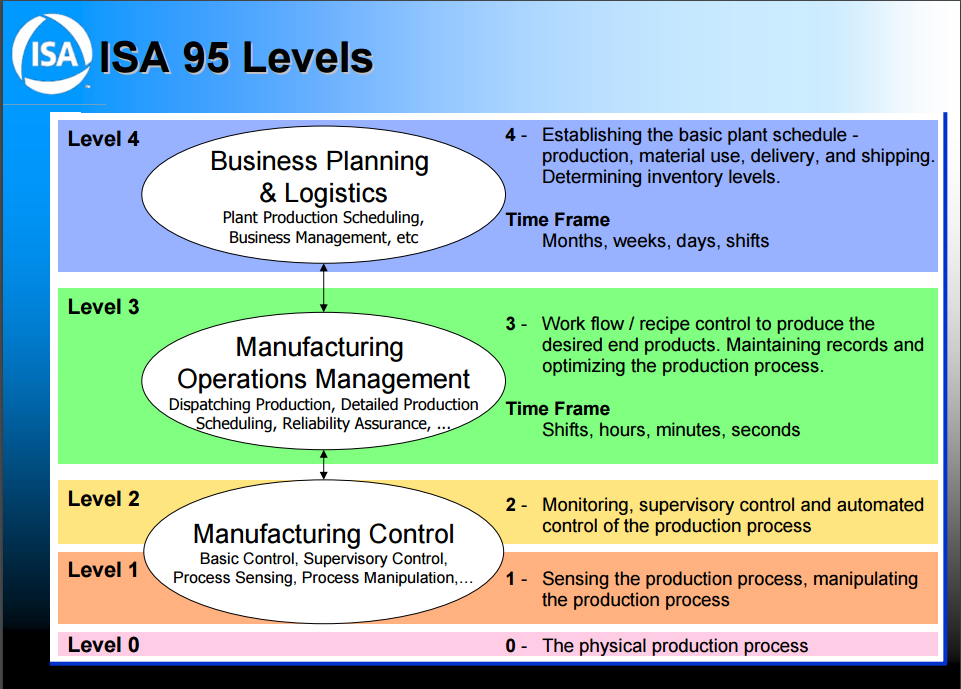
\includegraphics[width=0.9\linewidth]{img/ansi-isa-95}
	\caption{The manufacturing levels as described and defined by ANSI for the ISA-95 levels \citep{brandl2008ISA}. }
	\label{fig:ansi-isa-95}
\end{figure}

By creating an overview of the different layers in the manufacturing process, an understanding of how optimization problems in these layers can be solved with agent solutions can be given.



\subsection{Asset Management}
On the top of the ANSI structure is the overview of the manufacturing process, also known as Asset Management, which is the broad overview of the administration of assets. This includes the design, construction, use, maintenance, repair, disposal and recycling of assets. For most corporations and enterprises, the focus lies on the operational aspects of the assets, due to the fact that asset failures result in production or service delays. Therefore, insufficient asset management on the one hand results in loss of the asset itself, and on the other hand results in loss due to production delays and loss of service \citep{trappey2013multi}.  A lot is currently being researched, for example by \citet{leitao2009agent}, on asset management, and \todo[verbeteren]{verbeteren} especially the condition monitoring and prediction are well researched. This\todo[which]{which?} is due to the shift from reactive repair work to real-time condition monitoring, prediction, diagnostics and pre-scheduled maintenance. Also, traditional asset management approaches are poorly suited for current equipment failure solutions. %\Todo{Onderhoud + inspecction. Gebruik woord ``Asset Integrity''}
	
Traditional manufacturing control systems are unable to be sufficiently responsive, flexible, robust and reconfigurable due to the fact that they are built upon centralised and hierarchical control structures. These are optimal for perfect optimization, but weakly responsive to change. Another consequence of this structure is that a single failure can shut down an entire system \citep{leitao2009agent}. This requires a change to decentralized asset management, demanding new process control methods. \todo[Could be a possible solution for this problem]{Could be a possible solution for this problem}
	
Generally, researchers use agent-based technology to represent real world situations through the use of a computational simulation process, where agents can interact with each other to find a common goal. Typically, in these environments, agents have conflicting goals. In such circumstances, they will negotiate with each other in order to resolve conflicts \citep{rosa2009intelligent}. These methods will be described in \Cref{sec:negotiation}.
		
	
\subsection{Process Control}
One level lower than asset management is the order of process control, where there are three different processing methods: discrete, batch and continuous. Each process can be defined in terms of one or more of these methods. A discrete process method occurs when the production results in separate pieces. These are for example created in Industrial Robotic Solutions. Each robot produces a separate product in the manufacturing process. It is one of the most used manufacturing production applications. \todo[Tastbaar tengible example]{Tastbaar tengible example}

Batch production occurs when specific quantities of the materials have to be combined in particular ways. These are typically food production. An example is beer production. In a specific batch, the ingredients are combined, and after a period we have our required product.

The last process method is continuous production. This type of control is required if the variables are smooth and uninterrupted in time. The process of the creation of de-mineralized water is a continuous process. The water continuously flows through the system and results in the required product with no interruptions.

An example from \citet{engell2012optimal}, which is displayed in \Cref{fig:processstructure}, shows the typical process control method. This is in line with the ANSI standardisation described in \Cref{ch:intro}.

\begin{figure}[h]
\centering
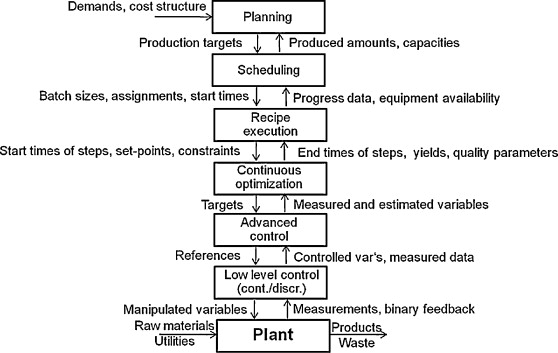
\includegraphics[width=0.7\linewidth]{img/process_structure}
\caption{Typical process structure from \citep{engell2012optimal}}
\label{fig:processstructure}
\end{figure}

\subsubsection{Planning and Resource Allocation}
When controlling a process, it is important to optimize the planning. The forms of decision making used in optimization of planning play an important role in the performance of a production plant. By using different mathematical and heuristic methods, the limited resources can be correctly allocated. This optimization is essential in order to achieve the objectives and goals of a company. By minimizing, for example, the time to complete the production, while satisfying the goals, efficiency is increased, which often results in cost reduction \citep{pinedo2005planning}.

An important aspect of the planning is the allocation of resources. One can optimize the production process, but without the correct resources at the right location at the right time, the optimization is limited. This is a crucial aspect of planning, which is often done manually in large production plants due to the often unexpected and complex decision-making processes involved \citep{pinedo2005planning}. By automating the resource allocation, a part of the overall planning can be automated.

Another large difficulty when planning, is that of ensuring that the assets are always operational, or that they have as short as possible planned downtime. This is achieved with predictive maintenance.

\subsection{Predictive maintenance systems}
To prevent malfunctions, maintenance is necessary.\todo[Planned and unplanned verwerken]{Planned and unplanned verwerken} However, this maintenance results in downtime, and is preferably left out, to keep operations running. This however results in the breakdown or wear-out of the systems. By maintaining assets before they break by so called ``preventive maintenance'' this damage can be controlled.

The old-fashioned model is corrective maintenance. Since maintenance results in the shut-down of production plants, most companies postpone the maintenance to the last moment possible. By ensuring to take as many hours as possible from the machine, the most is taken out of their investment. However, since the breakdown can happen any moment, such companies need a high inventory of spare parts and materials.  And usually the repair is more expensive than preventive maintenance.

Preventive maintenance is the alternative to corrective maintenance. Using predetermined fixed-interval planned maintenance, the assets are maintained. However, this results in uncertainty whether maintenance is planned too early, or worse, too late. How can one be assured that the maintenance timing is optimal, due to the many factors of influence on the asset (wrong usage, or external environment like sun, dust and rain)? Often either maintenance is done too soon, resulting in extra cost, or too late which results in the breakdown of the asset.

Condition-based maintenance is a step in the right direction. By ensuring preventive maintenance on the right moment, the machines do not break down and there is no overkill on maintenance. On specific intervals, the machines are measured regarding their current status and using, for example, vibration measurements or oil samples, their current condition can be assessed. Parts that have a high probability of failure can be replaced in their next maintenance or production stop. However, this is still not the optimal solution: measurements are sporadically done (not continuously) and there remains the chance of failure before the maintenance stop has occurred. \todo[threshold value]{Threshold value}

Using predictive maintenance it is possible to continuously, in real-time, monitor an installation. This can be done over a distance. Currently there are assets filled with sensors which produce data. This data is shared with people, other machines and servers. This allows for prediction of failures and real-time maintenance. \todo[Verschil tussen CBM \& PM]{Verschil tussen CBM \& PM}

Currently a lot of research is conducted on this new form of maintenance \citep{muller2008concept}. This central analysis is done by recognizing patterns in the data which allows for prediction of possible faults. This branch of maintenance is also known as e-maintenance \citep{yu2003multi}, or intelligent maintenance \citep{vermaak2007multi}.


\subsection{Real-time Monitoring}
To ensure that processes are running according to plan and that continuous planning is applied, real-time monitoring is required. Essential in implementing a real-time plan or schedule is that it has to be generated in seconds. This may be the case if rescheduling is required multiple times a day because of schedule changes. This can be done in two ways. The first way is to review the overall processes and functions performed on the data in real time through graphical charts and bars on a dashboard. This, however, requires manual input, or an algorithm that comprehends all the data. The second method is by implementing a programmable logic controller. By automating the industrial electromechanical processes in a predictable and repeating sequence by use of a logic ladder, a real-time controller is achievable. However, when using a programmable logic controller, the decision process is done on a very low level and optimization is difficult.

\section*{Manufacturing with Agents}
When dealing with multiple processes, in  production and manufacturing, and when having to keep real-time track of the assets with sensors, the most common solution lies in agent solutions \citep{leitao2013past, monostori2016cyber}. This is often easier said than done. In the following section, an introduction in agent solutions will be given with a focus on manufacturing. \todo[Brug duidelijker]{Brug duidelijker!}

\newpage
\section{Agent Solutions}
The new requirements in production ask for new manufacturing planning. This requires a new planning method, which is best implemented using distributed, decentralized structures \citep{parunak1999industrial}. The basis of a distributed method lies in object-oriented programming (OOP) and multi-agent structures. Using these structures in combination with communication, planning can be optimized. This structure is also similar to that of the ANSI. We have a high-level object which can consist of multiple lower-level objects. First some terms have to be discussed, after which we can link the manufacturing processes to the agent-based solutions.

\subsection{Object-Oriented Programming}

Object-oriented programming (OOP) is a programming method based on the concept of ``objects'', which may contain data and code. For example, an object can be a variable, a data structure, or a function, or a combination of these. The code that an object contains can be seen as the behaviour of the object, and as such it is easily interchangeable with an agent, since a method in OOP is an activity associated with an object. An object is made up of data and behaviour, which form the interface that an object presents to the outside world, and thus very similar to an agent \citep{shoham1993agent}.

Agent-oriented programming is a method often used to implement a multi-agent system, see \citep{mahar2012agent} for a thorough overview. In such a system anthropomorphic ideas, like beliefs, desires are used to model the objects, and thus called agents \citep{shoham1993agent}.% Import to note is that based on agent-based programming, see \citet{mahar2012agent} for a thorough overview, 

%\subsection{Convexity}

\subsection{Multi-Agent Systems}

Some terms used in the literature for data collection apparatus that aggregate the data are ``Smart Objects'', ``Intelligent Gateways'', ``Collaborative Networks'', ``Wireless Sensor Networks'' and ``Industrial Agents''. Most of these can be viewed as multi-agent systems (MAS) where the sensors communicate with one another as decentralized intelligent agents for independent action performance depending on the context, circumstances or environments (sensor input) of the situation. From such MAS, ambient intelligence  is conceivable: real-time decentralized decision making based on real-time data acquisition, analytics and negotiations. An example structure is shown in \Cref{fig:MAS_example}.

\begin{figure}[h]
	\centering
	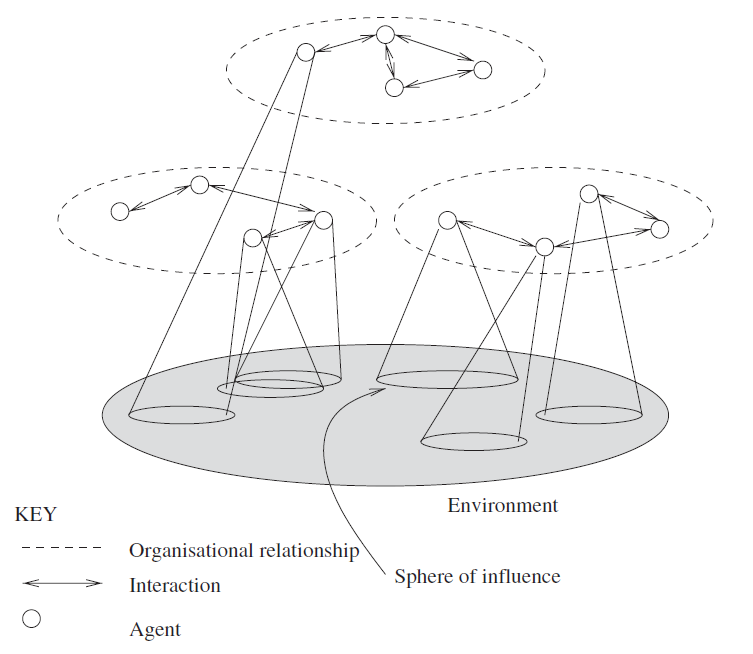
\includegraphics[width=0.7\linewidth]{./img/MAS_example}
	\caption{Typical structure of a multi-agent system \citep{wooldridge2009introduction}.}
	\label{fig:MAS_example}
\end{figure}

To define MAS, an agent needs to be defined more precisely. An agent is a system that is capable of independent action on behalf of its user or owner. As  \citet{wooldridge2009introduction} formulates it, ``An \textit{agent} is a computer system that is \textit{situated} in some \textit{environment}, and that is capable of \textit{autonomous action} in this environment in order to meet its delegated objectives.'' This independent action execution is already a form of intelligence \citep{wooldridge2009introduction}. In the MAS, the developer would most probably implement such intelligence by giving each agent ``Beliefs, Desires, and Intentions'' \citep{rao1995bdi}.  

Multi-agent systems (MAS) have been identified as some of the most suitable technologies to contribute to the deployment of decentralized optimization that exhibit flexibility, robustness and autonomy \citep{vinyals2010survey}. Currently there are a lot of relevant contributions regarding agent technologies to this emerging application domain. However, many challenges remain for the establishment of MAS as the key enabling technology \citep{vinyals2010survey}. A few problems, such as a lack of focus on multiple owners, decision making with only available local knowledge research and lack of collective sensing strategies, are still subjects that require extensive research. \citet{vinyals2010survey} see these as the possibly most active MAS research topics. Many of these problems can be solved with negotiation, which will be covered in \Cref{sec:negotiation}.

\subsection{Holonic Systems}
Another way of looking at agents, and more convenient in the manufacturing world, is by looking at MAS as holonic systems. Multi-agent systems are composed of autonomous software entities which allow them to be able to simulate a system or to solve problems. In manufacturing, the requirement linked to the real-time processes resulted in a new entity and control structure: holonic systems \citep{giret2005multi}. A holon is an intelligent entity, just like an agent, and able to interact with the environment. This allows the holon to take decisions to solve a specific problem. The holon has the property of playing the role of a whole system and a single part at the same time. The first successfully implemented holonic structure was created by \citet{van1998reference}. PROSA \todo[Waar staat Prosa voor?]{Waar stat prosa voor?} consisted of three types of basic holons: order holons, product holons, and resource holons. \citet{van1998reference} structured the system using the object-oriented concepts of aggregation and specialisation. By decoupling the system structure from the control algorithm, logistical aspects could be decoupled from technical ones. After they compared the holonic system with existing manufacturing control approaches, they concluded that the holonic system was able to cover all aspects of both the traditional pyramid and decentralized control architectures, meaning that it could be regarded as a generalisation of the two. 
\begin{figure}[h]
\centering
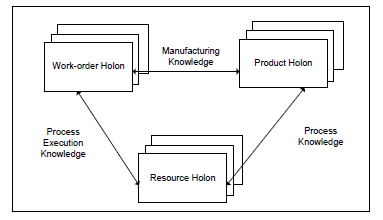
\includegraphics[width=0.7\linewidth]{img/holonic_manufacturing}
\caption{An example of an Holonic Manufacturing System (from \citet{giret2005multi}, based on \citet{van1998reference})}
\label{fig:holonicmanufacturing}
\end{figure}

The concept of holon is based on the idea that complex systems will evolve from simple systems more rapidly if there are stable intermediate forms, than if there are not. This means that the resulting complex systems will be traditional pyramids. However, although it is easy to identify sub-wholes or parts, holons do not really exist anywhere, making them decentralized \citep{van1998reference}.

\subsection{Task and Resource Allocation}
An example of resource allocation is when a set of agents shares a joint resource. Such a resource can be anything from indefinitely renewed continuous or discrete theoretical resource.\todo[Onduidelijk]{Onduidelijk} By limiting the use of the resource to one agent at the time, negotiation is necessary to ensure that all the agents can use the resource. The preference of the agent is often crucial. Since the agents have different preferences regarding the resource, it is possible and feasible to divide the resource and create a schedule describing who has access to the resource and at which time \citep{fatima2014principles}. 

The most common example of resource allocation is that of a pie. How should the pie be divided among the agents? Many strategies have been designed for solving this issue. Another example could be the allocation of energy. Which processor gets how much energy? These resources can be continuous or discrete.

The same principle applies to task allocation, where the agents want to achieve a common goal. To achieve this goal quickly, the agents must divide different tasks, which may overlap, and reach an agreement on the optimal planning. 

See \Cref{sec:negotiation} for the difference \todo[Added value]{Added value} in the task or resource allocation when dealing with negotiation.

\subsection{Scheduling and Planning}
Since most Process Planning and Scheduling (PPS) problems are NP-hard problems, many MAS have also been deployed to ``solve'' such problems in reasonable time. NP-hard (nondeterministic polynomial) problems are those problems which are at least as hard as the hardest problems in NP \citep{hromkovivc2013algorithmics}. This means that it is possible to reduce the problems in NP to the original problem, such as SAT (propositional satisfiability), in polynomial time. Using the decentralized global optimization approach, a (sub-optimal) solution can be found. This solution would be found faster than when using an (mixed) integer program~\citep{feng2014multi}. It does however depend on the practical application of the system to see whether it is an NP-hard problem. Furthermore, this \todo[What]{what} does not guarantee an optimal solution, rather that a reasonable solution will be found in reasonable time.

Real-world scheduling problems are usually complex and involve many approaches to find sub-optimal rather than optimal solutions using reasonable computing resources. This is often done using a mathematical programming approach. \citet{zhou2004bus}, try to use a MAS to heuristically solve the bus maintenance scheduling problem. It is shown that with equal optimality and less computing time without constraint violation, the MAS solution is comparable to the work of a mathematical programming approach.

It is also shown in \citet{bruccoleri2005production} that the agent-based approach outperforms the centralized mixed integer programming solution for the planning of a production.

Another example is the agile development with a MAS \citep{rabelo1999multi}. Agile development is based on the idea that requirements and solutions evolve through collaboration between self-organizing, cross-functional teams. Agile development promotes adaptive planning. By using a MAS for Agile planning, it has been shown that \textit{``the scheduling agility can be extremely improved once it is based on the following key points:
	\begin{itemize}%[i]
		\item
		distributed and autonomous systems instead of the centralized and non-autonomous solutions;
		\item 
		negotiation-based decision making instead of the totally pre-planned processes;
		\item
		application of different problem-solvers in the same environment instead of only one fixed problem solver;
		\item
		concurrent execution instead of the sequential processing''~\citep{rabelo1999multi}.
	\end{itemize}
}

Each agent is part of a heterogeneous system and processes its own information and has its own particular capabilities that it exchanges within the system. In this matter it contributes to finding a solution to the global problem, which works very well in complex environments. Optimization of scheduling in such complex environments is highly constrained; this is a context in which advanced analytics also has great difficulty. Using the dynamic, flexible and intelligent relaxation of the constraints within the distributed knowledge of the agents, autonomous intelligent decision making as a multi-agent system can be achieved \citep{rabelo1999multi}.

% A major difficulty with classical scheduling systems is handling of conflicts. Several problems can arise during the schedule generation, after its generation, and during its execution, such as the temporal, capacity, or technologic conflicts. These problems may come from the planning, scheduling or execution supervision activities. There are several methods that can be applied for the conflict resolution in a multi-agent system. HOLOS uses the Contract-Net Protocol coordination mechanism to support the task assignments to agents, and the Negotiation [7], [17] method to overcome conflicts taking place during one of the three mentioned scheduling phases \cite{rabelo1999multi}

%\section{Agent Technologies}

\section{Framework of a centralized and decentralized system}
When looking at the traditional pyramid, which is fully centralized, it seems difficult, if not impossible to translate this to a decentralized solution as shown in \Cref{lit:manufacture}. It should be possible to determine whether a centralized or decentralized solution, using a MAS or holonic system, should be implemented at a business process. A framework to compare a centralized versus a decentralised solution is discussed here. Essential in the difference between these two possible solution spaces is the location of the processing power for the calculations. Centralised solutions have a single control unit where the information flows to, while decentralized solutions do not have this structure.

A popular comparison, discussed by \citet{parunak1999industrial}, is that of the original Roman army structures. Decisions where made at the top and dripped down, while the information stream went up. This method has been deployed in most companies. Due to the fact that something can be computed on a single computer, and be optimized on this single program, an optimal decision can be found.

However, the increasing complexity of computer and information systems, combined with the increasing complexity of their applications, exceed the level of conventional centralized computing. This is due to the processing of huge amounts of data, or data that originate from different locations. To solve such difficulties, computers have to act more like agents where each agent can solve, or decide on part of the problem. This is where agent-based architectures are an ideal fit to such a decentralized organizational structure.

To push the decision making to the lowest level, excessive layers of management can be obsolete. This allows for, sometimes, easier to understand and developing of problems, especially if the problem being solved is itself distributed.

By using principles of decomposition which is a classical optimization (reformulation) method \citep{sharif2012yard} presents a comparative study of two contrasting approaches for modelling the yard crane scheduling problem: centralized and decentralized. It seeks to assess their relative performances and factors that affect their performances. They conclude that a centralized approach outperforms the decentralized approach by 16.5 \% on average, due to having complete and accurate information about future truck arrivals. However, since the decentralized under performs the centralized, the decentralized approach can dynamically adapt to real-time dynamic changes, making it better suited for real-life operations. 

To optimize these different types of resources allocation problems, there are different kinds of allocation problems, for which different solutions are feasible. The purpose here is to find what characteristics are optimal to use a centralized vs a decentralized solution.


\subsection{Size and Modularity}
A critical aspect of the possibility to determine whether a centralized or decentralised solutions is preferred is the search space size of the problem. The size of the problem is seen as the number of resources or task that have to be allocated.  If a clear structure is conceivable and a clear population is in place a centralized solution is infeasible. This is due to the global overview. However, the high sensitivity to size and complexity makes a centralized solution impracticable.

In a decentralized structure, individual models are decoupled from one another, errors in one module impact only those modules that interact with it, leaving the rest of the system unaffected. This can be seen in \Cref{fig:modularitydecentral-changeability}. It shows however the importance of having a clear modular problem. 

\begin{figure}[h]
\centering
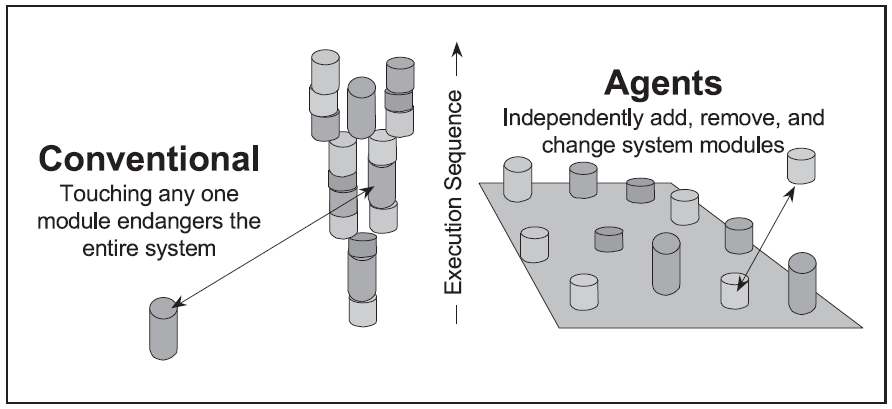
\includegraphics[width=0.7\linewidth]{img/modularity+decentral-changeability}
\caption{Comparison of a conventional control thread and an agent-based control, from \citep{parunak1999industrial}.}
\label{fig:modularitydecentral-changeability}
\end{figure}



\subsection{Dynamicity (Time Scale/Changeability)}
In a decentralized solution, the continuous monitoring of the state of the environment and typically the lack of complex decisions, a quick reaction to changes is possible. A high dynamical is the result. 

Unfortunately, it is difficult to achieve real-time scheduling in traditional manufacturing systems because the scheduling algorithms used are executed on a single, centralized computer that becomes computational incredibly difficult \citep{duffie1994real}.
\subsection{Solution Quality}
Since agent-based approaches are distributed, they do not have a global view of the entire state of a system. A lot can reached through communication and negotiation, but for a truly optimal solution, an entire view is necessary For example,  \citep{palmer2003decentralized} shows that this algorithm is not intended to find the optimal solution; it finds a good solution with less computation. 

In the centralized approach the assumption of a complete information on supply and demand is made. This requires rescheduling to adapt with changes. In the decentralized approach, no assumptions on the complete information is necessary. 


\subsection{Complexity}
Since an agent can execute actions only on its own surrounding, it is dependent on its local parameters. However, the agent can use information sent by its neighbours to adapt \citep{pujolle2006autonomic}. This interaction between the elements makes the complexity of a solution many times higher and more difficult than a centralized solution.

\subsection{Framework Overview}
Below a summary of the points above is given, with respect to the structure given. It is obvious that a decentralized solution is preferred, if the problem can be divided into sub problems. However, the real difficulty then lies in the complexity. Since in the system the communication becomes essential, the complexity increases.

\begin{tabular}{p{1.5cm} p{2.5cm} p{2.5cm} p{2.7cm}}
	\toprule
	& Centralised Solution & Decentralised Solution & Building Blocks\\
	\midrule
	Size / Modularity & Small; No sub-problems & Large; Ill-Structured; Easily dividable; Independent Modules & Population; Holonic; number of resources: (decision variables, parameters \& constraints) \citep{lang2015collaborative} \\
		\midrule
	Time scale and Changeability & Days - Weeks; Not subject to a lot of change & Real-time - Hour; Changeable  & Adaptive Capability ; Degree of Re- and Pro-activeness \citep{parunak1999industrial} \\
	\midrule
	Solution quality & Perfect & (sub-)Optimal & Object and Solution Space \citep{sharif2012yard} \\
	\midrule
	Complexity & Simple & Complex & Interaction between the set of elements; Communication \citep{pujolle2006autonomic} \\
	
	\bottomrule
\end{tabular}


\section*{Negotiation in a Decentralized Structure}
By decomposing the problem in smaller sub problems that a single agent can compute, and solve, the communication of the agents is essential. In order to integrate the solutions of the sub problems into the overall solution, the agents, which might not be cooperative, need to use negotiation.
%To achieve the autonomic-oriented architecture, we propose to select the appropriate control mechanisms among: 
%- adaptive: the agent adapts its actions according to the incoming events and to its vision of the current system state. The approach we propose is adaptive as the agent adapts the current control mechanisms and the actions undertaken when a certain event occurs. The actions the control mechanism executes may become no longer valid and must therefore be replaced by other actions. These new actions are indeed more suitable to the current observed state;
%- distribution: each agent is responsible for a local control. There is no centralization of the information collected by the different agents, and the decisions the agent performs are in no way based on global parameters. This feature is very important as this avoids having bottlenecks around a central control entity;
%- local: the agent executes actions on the elements of the node it belongs to. These actions depend on local parameters. However, the agent can use information sent by its neighbours to adapt the activated control mechanisms;
%- scalable: the proposed approach is scalable because it is based on a multi-agent system which scales well with the growing size of the controlled network. In order to adaptively control a new node, one has to integrate an agent (or a group of agents) in this node to perform the control. 

\clearpage
\section{Negotiation}
\label{sec:negotiation}
The negotiation of the agents in a multi-agent system has often been discussed above. This branch of research, also called automated negotiation, is studied by both artificial intelligence and economics \citep{jennings2001automated}. Concepts from fields such as decision theory and game theory are used in the design of appropriate negotiation and interaction environments \citep{jennings2001automated}. Negotiation is used to reach an agreement that meets the constraints of two or more parties in the presence of conflicting interests. And thus it is a basic means of getting what you want from others \citep{fisher1987getting}. It is back and forth communications designed to reach an agreement when you and the other side have some interests that are shared, and others that are opposed. Agents reason rationally and strategically. An agent's objective is to maximize the expected value of its own payoff. 

The four components of a negotiation model are~\citep{fatima2004agenda}:
\begin{enumerate}
	\item The information state of agents and domain;
	\item The negotiation protocol;
	\item The negotiation strategies;
	\item The negotiation equilibrium.
\end{enumerate}

Since negotiating situations occur when there is a conflict of interest, the first step will be to detect such a conflict. Agents will use communication channels and try to eliminate the conflicts. Conflicts may be about limited available resources, or ther may be a conflict between the beliefs of some agents. In the first case, optimization is the result, whereas, in the second case, one of the agents will have to change its beliefs \citep{shen2003multi}. Often negotiation is seen as maximizing the quality of the result. Two types of optimization are possible: one, the agents can try to achieve Pareto optimality, meaning that the outcome maximizes the product of the agents' utilities, or two, they try to reach a Nash equilibrium, meaning a stable state in the system. Both ways will be discussed in the evaluation of the model \Cref{ch:eval}.

Negotiation is done by exchanging messages among agents. Since the process involves several messages, a discussion will take place in which each agent's belief and goals will be an important factor. These depend on the global situation. Clearly, to be able to negotiate, agents must be able to reason. Thus, negotiation is restricted to cognitive agents. Automated negotiation is essentially a distributed search in the space of potential agreements between the different negotiators represented by autonomous agents, which involves the exchange of relevant information and aims to find an agreement that is acceptable to all participants.

\subsection{Negotiation Domain}

As discussed before, planning can be seen as concerning multiple different tasks, task allocation and resource allocation. The same holds for the negotiation domains, which can be divided into task oriented domains (TODs), state oriented domains (SODs) and worth oriented domains (WODs) \citep{rosenschein1994rules}. TODs are the simplest and an agent's activity is defined in terms of the set of tasks it has to achieve. It is assumed that all resources are unlimitedly available, and the advantage of negotiation is that it allows for the redistribution of tasks amongst a group of agents which can results in a more efficient task order. A typical example is that of mail delivery where an agent may carry another agent's mail at little extra cost. It is certain that the states come closer to a Pareto optimal solution as all agents can proceed with their original task list and be no worse off \citep{rosenschein1994rules}. 

SODs deal with problem where agents wish to change their environment from an initial state to some goal state. The classic AI Blocks World problem is a classic example. Here the agents have to place as many blocks vertically as possible. However, the catch is that the agents must sometimes remove a block to access another block. This gives the possibility of conflict and dead end, since the agents may have different goals, and it is not feasible to try to satisfy all these goals for all agents. This means that the agents must be able to make concessions in order to reach an optimum. These concessions can be in the form of a joint plan \citep{rosenschein1994rules}.

WODs are where agents attach a worth to each potential state, using for example a utility function. This allows more flexible goals to be set and allows concessions to be made on these goals. An example would be agents in a marketplace where the goal for a seller may be to obtain the highest price for $x$ within time $y$, while the buyer tries the to obtain the lowest price. There is again the possibility of conflict and deadlock, but now within a more complicated bargaining environment \citep{anumba2003negotiation, fatima2014negotiation}.

\begin{mdframed}[style = mystyle, frametitle = Utility Function]
A utility function is a way of mapping the desirability of a state to an agent. So the higher the utility of a state, the more desirable this state is. When making concessions, an agent accepts states that are less desirable. 
\end{mdframed}

\subsubsection{Negotiation States}
An agent’s information state describes the information it has about the negotiation game. There are two possibilities, states with complete information and those of incomplete information. The first category is basic and most common in research. In these games the players are assumed to know all the information about the rules of the game and the players their preferences. However, in the incomplete information category, information may be lacking about a variety of factors in the problem \citep{fatima2004agenda}. The incomplete information state is of course most common in applied negotiations since it is not possible to include all the possible information of the world. Furthermore, private utility functions can be desired to not give away ones intention.
\subsection{Negotiation Protocol}
Negotiation Protocol is the set of rules that govern the interaction and defines who are the actors of the negotiation, the states that characterize a trade (for example, when a negotiation has begins or ends), the events that determine the change of actors' status, and messages that can be sent by the actors in a particular state. This, however, is no easy task, since there is no one-size-fits-all solution. Some attempts have been made, by \citet{marsa2014problems} for example, and a collection of design rules which allow, given a particular negotiation problem, to choose the most appropriate protocol to address it. However, these problems are only determinable when (1) the negotiation domain, including the issues and possible issue values, (2) a scenario utility histogram, which defines the distribution of the scenarios, and (3) several structural parameters that specify the configuration of each agent's utility function are known.

A typical negotiation protocol is very similar to that of our negotiations in our everyday life and work. Thus, a negotiation typically proceeds over a series of rounds, with one or more proposals being made at each round. It also includes the rules that impose the constraints on the proposals and the rule that shows when a deal has been struck \citep{fatima2014principles}. Different negotiation mechanisms need to be developed to suit the different application environments of a MAS. Unlike the negotiations between human beings, which involve more complex human interactions than those about simple technical issues, the negotiation mechanisms between agents are rule-based or case-based due to these clear protocols. However, the human negotiation approaches and theories, which mainly include game theory and human behavioural theories, provide a proper foundation for the negotiations between agents. 

The most important protocol is that of the alternating-offers protocol \citep{rubinstein1982perfect}. It is based on a divisible pie, discrete or continuous, and is the most widely studied among game theorists as well as MAS researchers \citep{fatima2014principles}. Each agent is allowed to make a single offer, and the proposal that yields the higher product of all the utilities of the agents is accepted. The best strategy that agents can follow in this protocol is to propose the agreement that is best for themselves amongst those with maximal product of utilities. Essential however is that the utilities of the other agents must be known to ensure that the maximal product of utilities is calculated. Another example is the contract net protocol (explained in \Cref{sec:lit:neg:multilateral}). 

The most common protocol to ensure concession is the monotonic concession protocol. It is a proposal which has also been adapted for multi-lateral negotiation in \citep{endriss2006monotonic}, and can cope with different strategies.

\subsection{Negotiation Strategies}
A negotiation strategy can be defined formally as an apparatus which allows the agent to determine the content of the action that it will perform consistently with the protocols. In general, for a given set of negotiation protocols there are many strategies compatible with it, each of which can determine a different action. This means that a strategy can work well with a given protocol, but does not work with others. So, the choice of strategy depends on the protocol in use and on the negotiation scenario \citep{di2015multi}.

Often these strategies are private, meaning that not all the agents can see what the strategy of an agent is \citep{fatima2004agenda}. 

\subsubsection{Concession Strategy}
\label{sec:concessionstrat}
When negotiating, it is essential for the agents to make concessions, only in TODs it is unnecessary, as explained. Initially each of the agents involved makes a proposal that has the highest utility to itself. If no concessions are made, the agents will never reach an agreement. By making concessions on the utility, a proposal towards the agents agreement-zone can be made, which is essential in finding an agreement. Furthermore, as put by \citet{endriss2006monotonic}: a concession should always be minimal with respect to the utility loss incurred by the agent making the concession.

\begin{definition*}[Reservation curve and Agreement zone]
	When an agent has an utility, it usually has a minimum value to which is will concede. This curve of all points that have the minimum utility vallue is called the reservation curve. 
	
	Multiple agents have different reservation curves.
	\todo[insert figure!!]{Make figure}
		
\end{definition*}

\begin{figure}
		\begin{tikzpicture}
	\coordinate (v1) at (0,0) {};
	\node (v2) at (0,5) {};
	\node (v3) at (5,0) {};
	\node (v4) at (2.5,2.5) {Agreement-zone}
	\draw[->]  (v1) -- (v2) node[left] {Issue 1};
	\draw[->]  (v1) -- (v3) node[below] {Issue 2}; 
		\draw[name path = C] (5,1) .. controls (3,1) and (1,3) .. (1,5) node[right] {Reservation Curves};
	\draw[clip, name path = B] (0,4) .. controls (2,4) and (4,2) .. (4,0) ;
	\begin{pgfonlayer}{bg}
	\fill [gray!50,
	intersection segments={
		of=B and C,
		sequence={L2--R2}
	}];
	\end{pgfonlayer}
	
	\end{tikzpicture}
\end{figure}
When dealing with how to concede, there are multiple strategies. Most of these are one version or another of a monotonic concession protocol, meaning that the desired utility of the agent will never increase. This means that the desired utility will always decrease, or stay the same. After each proposal, there are two options. Either the agent refuses to make a concession and sticks to the previous proposal or it makes a concession and proposes a new deal that is less preferable to the agent. The monotonic concession protocol is verifiable, and guaranteed to terminate. This is due to the conflict deal that would occur if no agents concede, which gives both agents a utility of 0 \citep{endriss2006monotonic}.

%Using the monotonic concession protocol, negotiation is guaranteed to end (with or without agreement) after a finite number of rounds. Since the set of possible deals is finite, the agents cannot negotiate indefinitely: either the agents will reach agreement, or a round will occur in which neither agent concedes. However, the protocol does not guarantee that agreement will be reached quickly. Since th

There are multiple options when dealing with concession to a multilateral negotiation \citep{endriss2006monotonic}. Most of these have a relation to social welfare concepts, meaning that the agents will together try to maximize the utility of all the agents. This means however that the utilities of the other agents must be know since, it is not possible to discover the group maximum using private utilities.

Four concession strategies are given by \citet{wu2009efficient}: 
\begin{description}
	\item[Amount of utility] an agent concedes a fixed amount utility per time. 
	\item[Fraction of utility] an agent concedes a fraction of the desired utility. 
	\item[Fraction of the difference] the agent concedes a fixed fraction of the change in current desired utility and a reference point. 
	\item[Fraction of remains] the agent concedes a fixed fraction of the issues that no agreement has been made on yet. \end{description} 
\citet{wu2009efficient} found very little difference between the performances (distance from Pareto-optimum) of the concession strategies, although the fixed step was the quickest. 

\begin{definition*}[Social welfare]
	
\end{definition*}
When dealing with private utility functions matter change completely. There is no way knowing whether the other agents has conceded. A solution to this is proposed by \citet{zheng2015automated} using the reactive concession protocol.

\subsubsection{Reactive Concession Protocol}
The reactive concession protocol as proposed by \citet{zheng2015automated} tries to solve the problem that occurs when dealing with private functions and ensuring that there is not one agent that does not stall its concessions. \citet{zheng2015automated} show that by having an agent concider its own utility change resulting from another agents' offer, it can concede accordingly. There are two cases. If the change in utility that the other agetns' offer caused has resulted in an higher utility than the reservation utility, the agent will respond with the non-reactive concession strategy. 

However, if the utility is lower than the reservation utility, the agent will concede by an amount based on the change the agent perceives. By checking the last best offer, the agent checks for the marginal perceived change of utility and the total perceived change from the original offer. This gives two values, of which the maximum will be the agents' concession. Exact details will be discussed in \Cref{sec:reactiveconcessionstr}.


\subsection{Evaluation and Equilibrium Solutions}
When evaluating the dilemmas of a negotiation between agents, it is essential to determine the Pareto-Frontier. Visualized in \Cref{fig:paritooptimal}, it is used to determine whether an outcome of a negotiation is efficient. This means that no improvement can be achieved for all agents. In the figure we have the utility of $\text{agent}_\text{i}$ plotted against that of  $\text{agent}_\text{j}$. In the set of all possible outcomes, lie all the possible agreements, which are all offers, that are acceptable by both agents.

\begin{figure}[h]
	\centering
	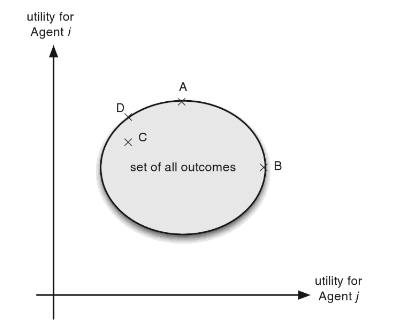
\includegraphics[width=0.7\linewidth]{img/parito_optimal.png}
	\caption{An example of Pareto optimality. Locations A and B are optimal, since no improvement for at least one agent, without loss for the other agent, is possible. C and D are not optimal since they utility of the agents can be increased. From \citet{fatima2014principles}.}
	\label{fig:paritooptimal}
\end{figure}

An offer is Pareto optimal if the agents cannot choose an new offer for which at least one agent has a higher utility, while the other agents have the same utility. In the figure these are shown as $A$ and $B$. Each other offer for these agents decreases at least the utility of one of the agents. Offers $C$ and $D$ are not Pareto optimal since both offers can be improved for at least one agent. The line of points in which an improvement of utility for one agent necessarily means a decrease in utility for the other agent is the Pareto-Frontier. 

Formally: If we have agents $M = \{1,...,m\}$, and issues $N = \{1,...,n\}$ denoted as issue $j\in N$, than an offer $x = \{x_1, ..., x_j\}$ is Pareto optimal if the outcome of negotiation $x$ has no feasible allocation $x'$ such that $ \exists i, u_i(x')> u_i(x) \in M$, while $\forall i, u_i(x')\geq u_i(x)  \in M$. 

The Nash equilibrium is the best reply to the other players strategies. This means that if both players play their Nash strategy, neither will have the incentive to change their method. Different equilibria are possible and shown in \Cref{fig:majorcategoriesofgametheory}. 

\begin{figure}[h]
	\centering
	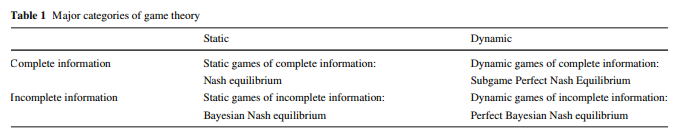
\includegraphics[width=0.9\linewidth]{img/major_categories_of_game_theory}
	\caption{The four types of games in game theory from \citet{trappey2013multi}.}
	\label{fig:majorcategoriesofgametheory}
\end{figure}
The most common Nash equilibrium and probably most widely known is that of the prisoners dilemma:
There are two subjects of a crime, agent $i$ and $j$. However, the evidence is not very convincing and therefore the prisoners are interrogated separately. If both confess, they get three years of prison. If both do not confess, they get a lighter sentence of 1 year. Finally, if one of them confesses to the crime and the other does not, the confessor will be freed, and the other will be jailed for five years.
This can be visualized in a normal form pay-off matrix. It is common to refer to confessing as defection, and not confessing as cooperating.
\begin{table}[h]

\begin{tabular}{|c|c|c|c|}
	\hline 
		&  				& \multicolumn{2}{c}{Agent $i$}\\ 
	 	&				& defect (confess) 	& cooperate ($\neg$ confess) \\ 
	$Agent j$	& defect (confess)	&  	(-3, -3)			& (0,-5) \\ 
		& cooperate($\neg $ confess) 	&  (-5, 0)				& (-1,-1) \\ 
	\hline 
\end{tabular} \label{tab:nashprison} \caption{The prisoners dilemma}
\end{table}
For agent $i$ it is obvious to reason as follows. Suppose agent $j$ cooperates. Then the best response is to defect. Suppose the agent $j$ defects. Then the best response is to defect. In other words, defection for agent $i$ is the best response to all possible strategies of the player j. This makes defection the dominant strategy for agent $i$. Since both agents reason the same way, the agent will both defect which results in the Nash equilibria (defect, defect).

In general, that two strategies $s_1$ and $s_2$ are in Nash equilibrium if: under the assumption that agent $i$ plays $s_i$, agent $j$ can do no better than play $s_2$, and under the assumption that agent $j$ plays $s_2$, agent $i$ can do no better than play $s_l$. Thus strategies $s_i$ and $s_j$ for agents $i$ and $j$ form a Nash equilibrium if they are the best response to each other  \citep{wooldridge2009introduction}. 

Important to note here is that in the prisoners dilemma, the Nash equilibrium is the only solution which is not Pareto optimum.  THe optimal social solutions, which is if both agents do not confess, is different from the Nash equilibrium.  Furthermore, it should be stated that not every interaction scenario has a Nash equilibrium and some interaction scenarios have more than one Nash equilibrium. 
\subsection{Principled Negotiation}
\label{sec:principlednegotiation}
An example of a common method for negotiation is principled negotiation. This method developed by \citet{fisher1987getting} was founded on the idea that negotiators could reach better agreements by finding favourable agreements. By focussing on interests not positions and using objective criteria, an agreement is more likely to be reached. This method has successfully been deployed in a multi-agent system for air traffic management \citep{wangermann1998principled}. \citet{fisher1987getting} emphasize the fact that it is important to agree on objective criteria for assessing options \citep{fisher1987getting}. If an agreement can be reached using this criterion, it is more likely that it is rational. Furthermore, principled negotiation is useful for systems in which no agent has global knowledge of the system.

%The purpose of this type of negotiation is to help to reach agreement without jeopardizing the business relations. It was created by \citet{fisher1987getting} and they refer to this kind of agreement as a wise agreement. Wise agreement is agreement that meets the interests of both parties to the extent possible, is long lasting, and also considers the interests of the larger society. The basis of this negotiation principle is to separate the relationship issues from the problem issues, to focus on interests not on positions, while trying to be creative in developing solutions.

% \cite{wangermann1998principled} Principled NegotiationI was developed as a method that negotiators could use to reach better agreements than could be obtained using traditional confrontational tactics. The underlying idea is that in most situations there are options that will benefit all the parties in negotiation. A favorable agreement is more likely to be reached if a negotiator proposes options for mutual gain and if all the parties assess the options using objective criteria (Fig. 3). Traffic management agents would be able to a.pprove many of the proposals, as the proposing agent would try to ensure that the options provided mutual gain. 






%\subsubsection{Example}


%\todo{Breder trekken qua literatuur}%In a cooperative negotiation, agents are allowed to communicate and to receive side payments. Furthermore, in cooperative games, agents can make binding commitments. These cooperative games result in coalitions which can be used to solve some of the problems that occur from the prisoners dilemma. 

%Within negotiation there are several more methods~\cite{wooldridge2009introduction}:
%\begin{itemize}
%	\item Patient players;
%	\item Impatient players;
%	\item Negotiation decision functions.
%\end{itemize} All these methods can be used to negotiate/bargain for resource allocation. More examples are available which will also be analysed in the in-depth literature review.

%Several other communication techniques might be useful for decision making~\cite{wooldridge2009introduction}:
%\begin{itemize}
%	\item
%	Arguing;
%	\item
%	Public vs private announcement;
%	\item
%	Contract net protocol \cite{smith1980communication}.  
%\end{itemize}

%Contract net protocol is a form of cooperative distributed problem solving that will be discussed in the scheduling section (\Cref{sec:AIscheduling}).
%\subsubsection{Framework}
%An overview of these different methods is in Fatima et al.~\cite{fatima2014principles}. Unfortunately this book is still lacking. 
\subsection{Negotiation using a Mediator}
A mediator can be used when negotiating, like is used in typical hierarchy, voting, and auction based negotiations. 

Voting is a form of group decision making. The agents participating in the voting will take into account their own preferences as well as those of others when making decision about how to vote. This will often have a strategic flavour. By aiming to rank or order the candidates, a group decision can be made.

Another option are auctions, a popular mechanism to reach an agreement within the allocation of resources to agents. Examples include English auctions, Dutch auctions, Vickrey auctions and First-price sealed-bid auctions \citep{wooldridge2009introduction}. Interaction between a large number of low-level agents results in a complex system behaviour which is difficult to understand, to control and to predict. Structuring the agents in a hierarchy is the appropriate solution to tackle this complexity \citep{van1998reference}.

However, in mediated negotiation, the agents have no desire to make concessions, and an (sub-)optimal solution cannot be guaranteed.

\subsection{Mapping of Negotiation Protocols}
An attempt at the visualization of the different negotiation techniques is strived at. Three variables are decided on. Single- vs Multi-Issue negotiation; bi- vs multi-lateral negotiation, and; perfect vs imperfect information negotiation.  
\begin{figure}[h]
	\centering
	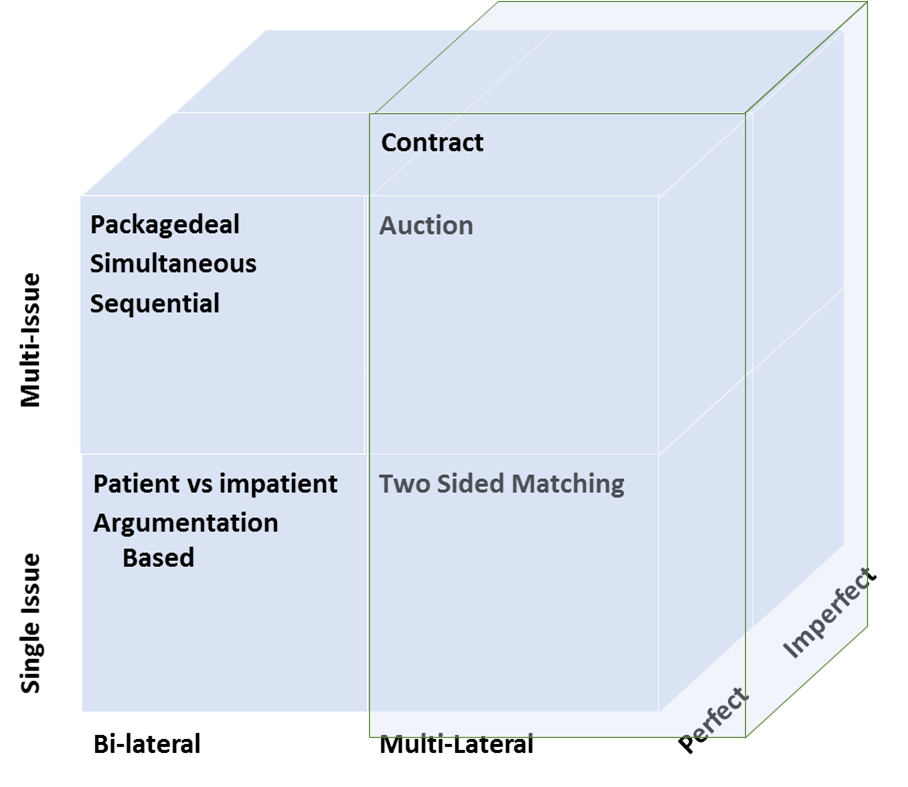
\includegraphics[width=0.7\linewidth]{img/mapping_nego}
	\caption{Overview of the negotiation protocols used, and researched in the literature. The usage of an proposal based protocol for a multilateral multi-issue situation is missing in the manufacturing literature.}
	\label{fig:mapping_nego}
\end{figure}


\begin{figure}[h]
	\centering
	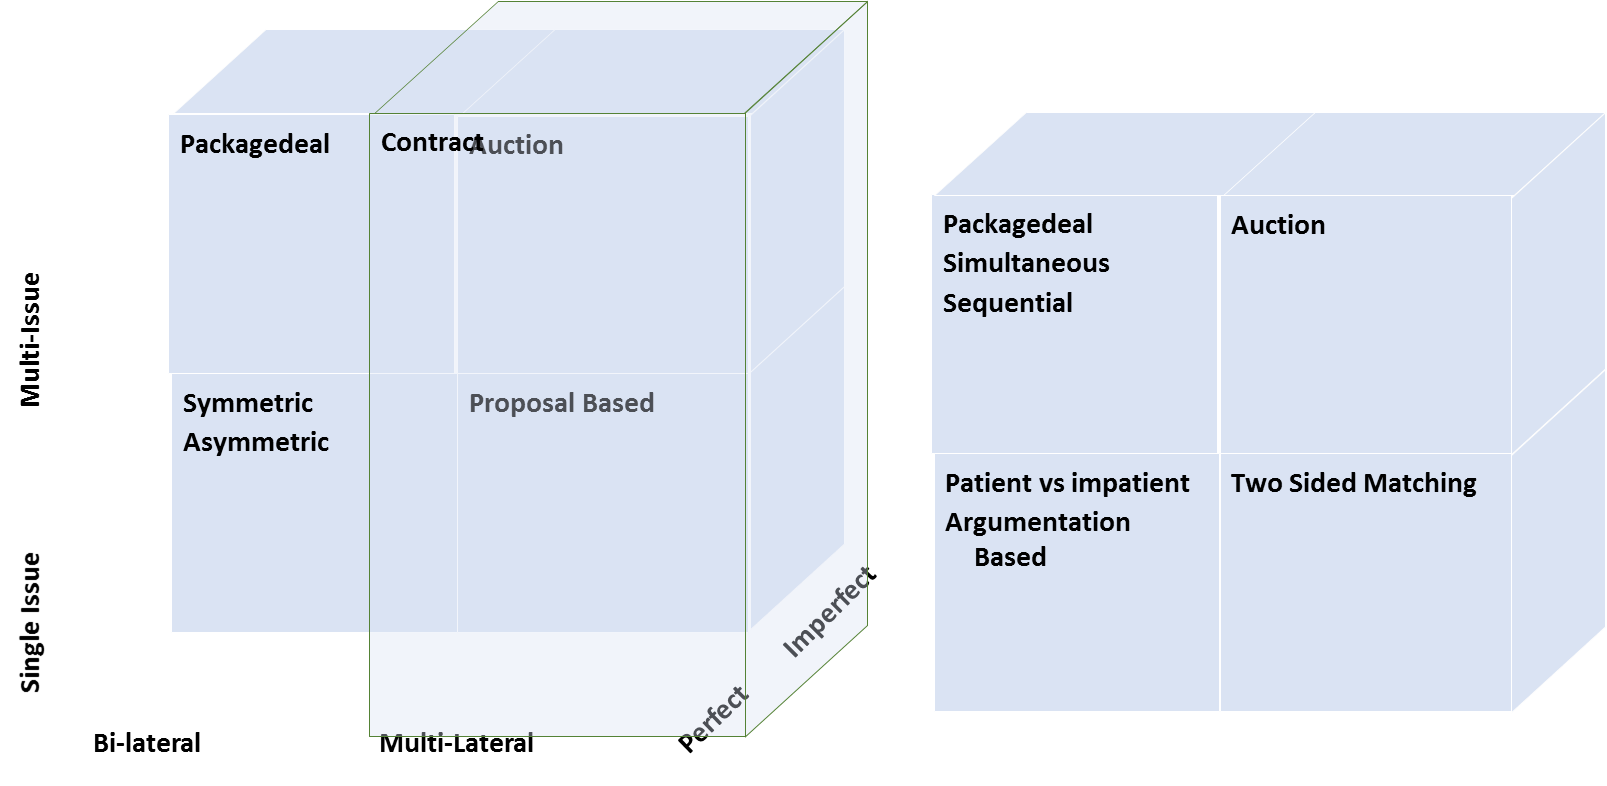
\includegraphics[width=0.9\linewidth]{img/mapping_nego2}
	\caption{For completeness, the same figure as in \Cref{fig:mapping_nego}, but with the display of the imperfect information protocols.}
	\label{fig:mapping_nego2}
\end{figure}

\subsubsection{Single-Issue}

Negotiation among self-interested agents has been studied from the perspective of game theory. This is most obvious when the agents negotiate on single issues. An example might be the price of a product. When dealing with a single issue there is only one goal for both agents and there must be a conflict. If there was no conflict, no negotiation would be necessary. Typical single issue methods are patient vs impatient players, two sided matching. Argumentation based methods, which are based on the beliefs of an agents are also included in the mapping.

Essential is that all these methods are a form of the alternating offers protocol. Depending on the sort of players, the method result in completely different behaviours. These negotiations can either be complete or incomplete meaning that all information is known, or not all. 

When the game is complete, all the agents know all the information about their states and the strategies of other agents. When not all is known, the game is incomplete. The idea of negotiation is that we have an incomplete game, since if the strategies are known, most negotiation would not be necessary.

When looking at perfect vs imperfect information, it means that either the information states of the agents is perfect, meaning that the agent is perfectly informed of all the events that have previously occurred and actions (like chess), or that not all actions are known. Depending on the implementation of the system, with for example public and private announcements, the difference is made. 

When looking at single issue negotiation, depending on whether the negotiation happens between 2 (bilateral) or more (multi-lateral) agents, there are a few protocols possible. Bilateral negotiation can be either patient or impatient \citep{fatima2014negotiation} meaning that an agent has a initiative to limit the time of negotiation. Most negotiation in the manufacturing are time restrained, thus impatient agents must be implemented \citep{kraus1995multiagent}. In symmetric vs asymmetric the players are uncertain about the other players utility functions (as is the case in imperfect negotiation), but essential is that one agent might know more than the other in the asymmetric protocol.

\subsubsection{Multi-Issue}
 When negotiating multi-issues, agents attempt to combine 2 or more issue in their discussing. An example is the typical seller, buyer relationship between two agents, as for example shown in \citet{schramm2013bilateral}. Here a supply chain construction company is used to asses an method to support bilateral negotiation. Aspects like price, quality and lead-time are considered as issues, on which can be negotiated. Most used multi-issue method, for single-lateral negotiation is the package deal method. In this method, complete packages with all the issues are provided. These can be discussed either sequentially or simultaneously. 

 \begin{figure}[h]
 	\centering
 	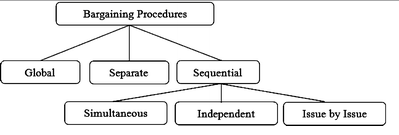
\includegraphics[width=0.7\linewidth]{img/multi-lateral}
 	\caption{An overview of the different negotiation method for multi issues bargaining. From \citep{abedin2014agenda}.}
 	\label{fig:multi-lateral}
 \end{figure}
 
 Agents can employ either an issue-by-issue (one-at-a-time) approach, or a packaged approach in the negotiation agenda \citep{fatima2004agenda}. \citet{abedin2014agenda} think that a packaged approach is optimal since the agent lack knowledge about the opposing agent. As one issue is settled, the agent subsequently negotiates the other pending issues. This allows the agent to be cautious and opportunistic at the same time.
 
 When choosing the preferred method of negotiation, important to realize is the solution required. As explained above,\citet{abedin2014agenda} says that the issue-by-issue approach has a higher chance of obtaining the Pareto optimal solution. However, since the utility of an offer is not simply a sum of the utilities of the individual issues, some prefer to use the package deal \citep{zheng2015automated}.

%The majority of the existing work on multi-issue negotiations focuses on the negotiation strategy, assuming the agenda and the procedure to be predetermined \citep{fatima2004agenda, lai2004literature}. Interesting to determine would be the influence of the domain and protocol since, depending on the scenario under which the negotiation is taking place a supervised agenda procedure can have a positive impact on the outcome of the negotiation when compared to a procedure without use of an agenda \citep{abedin2014agenda}.


% 
 %The agenda based approach specifies how the issues will be settled. Agents can employ either an issue-by-issue (one-at-a-time) approach, or a packaged approach in the negotiation agenda (Fatima et al. 2004). We have adopted the former; negotiation one issue at a time. The main reason for this is lack of knowledge about the opposing agents. As one issue is settled, the agent subsequently negotiates the other pending issues. This allows the agent to be cautious and opportunistic at the same time. For a multi-issue negotiation under incomplete information settings, the ideal solution is one that is Pareto optimal. A solution is said to be Pareto optimal if no agent can be better off without sacrificing the other’s utility (Wilkes 2008). So the proposed negotiation approach should be able to generate Pareto optimal solutions for multi-issue negotiations. The majority of the existing work on multi-issue negotiations focuses on the negotiation strategy, assuming the agenda and the procedure to be predetermined (Fatima et al. 2004; Lai et al. 2004). Depending on the scenario under which the negotiation is taking place a supervised agenda procedure can have a positive impact on the outcome of the negotiation when compared to a procedure without use of an agenda. \cite{abedin2014agenda}

% Issue by issue negotiation gives a high probability to find a negotiation zone in an incomplete information setting rather than package and simultaneous approach. In package and simultaneous negotiation approach, the agents have limited confident and information about each other, the issues, offers and preferences. With issue by issue negotiation, there can be different agendas. Generating the optimal agenda for both agents helps to maximize their utilities. A simple but useful interdependency mechanism is derived to handle the correlation between the issues. \cite{abedin2014agenda} 

% First, in a multi-attribute negotiation the preference of an agent over multiple issues can be complex. A traditional way to deal with this is to characterize the preference with a utility function (a mathematical formula) and agents make decisions based on this utility function. However, it is not trivial for a human to construct such a utility function over multiple issues, especially when preference over one issue is impacted by the values of other issues; thus, preference elicitation may take a long time or sometimes be intractable. Second, in a multi-attribute negotiation the solution space is n-dimensional (n>1) rather than a single dimensional line as in a single-attribute negotiation. This makes the negotiation strategy in multi-attribute negotiations complex: because the space is ndimensional, every time an agent plans to concede, she needs to first decide the direction of concession. Apparently there are many choices on the concession direction she can take: to concede on issue 1, …, n or different combinations of the issues. Specifically, the decision on the concession direction may also depend on the opponent’s preference because conceding on the issue more important to the opponent can make the offer more acceptable. Finally, to decide how much to concede is now more complicated because the direction can impact the amount as well. So the burden of computation and reasoning for the negotiation strategy is higher in a multi-attribute negotiation than in a single-attribute negotiation. Third, as mentioned above, in multi-attribute negotiations there exist “Win-Win” situations. For rational agents, they should not “leave extra money on the table”. In other words, the ideal result for the system is to realize a Pareto-optimal (or Pareto-efficient) solution. A Pareto-optimal solution is one which cannot be improved further without sacrificing someone’s utility, i.e. if there is another solution from which one of the agents can get more than from this Pareto-optimal solution, then the other agent must get less by that other solution. We say a multi-attribute negotiation model is efficient when agents will reach a Pareto-optimal agreement in the negotiation, if there exists a zone of agreement. \cite{lai2004literature}

\subsubsection{Multilateral}
\label{sec:lit:neg:multilateral}
The most common used method for multilateral negotiations are contract based methods, most popular being the contract net protocol. Contract net protocol by \citet{smith1980communication} is based on the principle that agents, each with a distinct expertise, can solve sub problems that are required to solve the global problem. This form of cooperative distributed problem solving is based on the assumption that agents in a system implicitly share a common goal, and thus that there is no potential for conflict between them.

Each agent, called a manager, that has some work to be subcontracted, broadcasts an offer and waits for other agents, the contractors, to send bids. After some delay, the best offers are saved and contracts are allocated to one or more contractors who process their subtasks. The contract-net protocol provides for coordination in task allocation. 

The protocol is best suited to problems in which it is appropriate to define a hierarchy of tasks. Since such problems allow to be decomposed into a set of relatively independent subtasks, there is little need for global information or synchronization. These subtasks can be assigned to separate agents. The contract net protocol main contribution is the mechanism that it offers for structuring high-level interactions between nodes for cooperative task execution \citep{smith1980communication}. With these contracts task allocation is possible. The allocation of resources gives difficulties however. 

Since the contract net protocol has the uncertainty of matches being stable, the protocol of two-sided matching has been developed. Furthermore, it is not certain that the matches are Pareto optimal. Using the two sided matching method, this uncertainty can be avoided, however, this protocol is harder to implement due to the fact that a clear allocation division is required. \citep{fatima2014principles}.
 
If the game is imperfect two sided matching does not work, and a proposal based protocol is the right fit \citep{rahwan2003argumentation}.

%\todo[Example of the three agents and three resources]{Example of the Three agents and three resources, }


%\subsubsection{Reasoning about ones interest}
%Interest-based negotiation (IBN) is a form of argumentation-based negotiation in which agents exchange (1) information about their underlying goals; and (2) alternative ways to achieve these goals \cite{rahwan2009formal}. 


\subsubsection{Heuristic methods in Negotiation}
\label{sec:lit:learn}
Most of the negotiation in manufacturing can be seen as multi-lateral multi-issue negotiation. Three important distinctions are to be made, based on \citet{lai2004literature}. 
\begin{enumerate}
	\item
	issue by issue negotiation;
	\item
	multi-issue cooperative negotiation;
	\item
	multi-issue negotiation with heuristic methods.
	\end{enumerate}
	
	The first aspect looks at the agreement which is built through a strategy, and examines this individually and interactively, and the parties are considered as non-cooperative and they are built for environments with incomplete and asymmetric information, where an agenda containing the order in which issues are treated is needed. For the second aspect a multi-issue concession strategy is used whose parties are considered cooperative and they have complete and symmetrical information about their environments. These two aspects have been discussed in the sections above. In the last type, an agreement is reached through a hybrid negotiation strategy, which uses the first two types of theoretical framework with the focus in automated models based on autonomous agents for multi-issue negotiation and in negotiation strategies tractable. This is also where possible learning methods are available \citep{schramm2013bilateral}. 
	
	These heuristic methods are a lot more common in the implementation of negotiation, as discussed by \citet{leitao2013past, monostori2006agent}, since it does not require the through analysis of the states and protocol compared to the game theoretic methods. Also it allows for larger groups and learning in the agents.
	
\subsubsection{Learning methods in Negotiation}
When dealing with heuristic methods for negotiation, learning methods can be implemented. An overview can be seen in \Cref{fig:negotiationlearning}. 

\begin{figure}
\centering
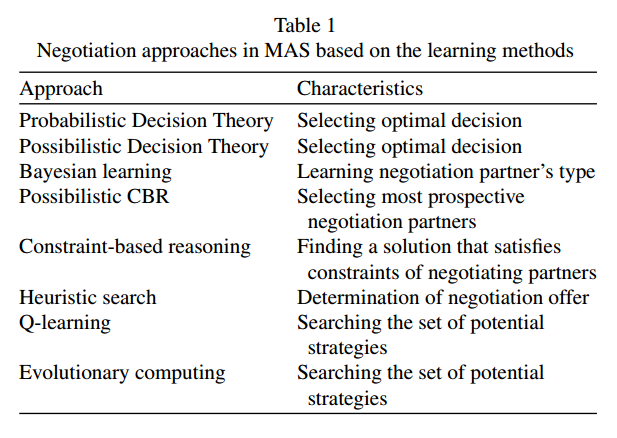
\includegraphics[width=0.7\linewidth]{img/negotiation_learning}
\caption{Overview of different learning methods for heuristic negotiation methods from \citet{beheshti2014homan}}
\label{fig:negotiationlearning}
\end{figure}
Based on the research conducted on heuristic methods and \citet{jennings2001automated}, it can be concluded that the optimal research in learning in heuristic methods is not yet known. They are often used however to decide on the optimal counter bid in \citet{beheshti2014homan}. They show that efficient learning algorithms based on an statistical ranking algorithm and linear regression, all with linear time complexities. These characteristics allow our method to be used in real-world applications. 
\section{Negotiation in Manufacturing}
There are many applications of agent based solutions in the manufacturing world \citep{monostori2006agent}. In these negotiations an overwhelming aspect is realised in the creation of intelligent individual agents, and less on the overall intelligence of the system. Often ignored is the specific negotiation method in these systems. This is where the problem lays, since conflicting interest, essential in the optimal decision making, are left out. An example where these conflicting interest are well implemented is in \citet{zheng2014cloud}. A cloud consumer usually prefers a high reliability, whereas a cloud provider may only guarantee a less than maximum reliability in order to reduce costs and maximize profits. If such a conflict occurs, a Service Level Agreement cannot be reached without negotiation. Automated negotiation occurs, when software agents negotiate on behalf of their human counterparts.  

%Many negotiation solutions have been ``invented'' but little has been truly applied in the manufacturing world \citep{leitao2009agent}. 

Rockwell Automation uses agents in its automation processes and is one of the industrial leaders in the implementation of agent based solutions \citep{vrba2011rockwell}. One of their future insights in the requirements of agent based solutions is to enhance the capabilities of agents for expressing and exchanging knowledge, and as a consequence, to increase the flexibility of control systems. In order to correctly do so, better insights in the negotiation is needed.

Overall, nearly all factory scheduling negotiations use some form of these market-based approaches \citep{monostori2006agent} to implement the solutions. Different version of the contract net protocol were used or other auction based methods. The problem with these methods is that no reasoning about another's interest and desires is achievable. If this is known, more efficient and better systems can be achieved. It is however shown in \citep{bruccoleri2005production} that the agent based approach using market auctions out performs the centralized mixed integer programming solution. This system uses bilateral simultaneous negotiation on the medium level of the production plant. It is however a form of auctions, where the agents simultaneously bid towards the goal. If this system already outperforms a centralized system, a non-auction based method might outperform even better.

Other examples of negotiation in a multi-agent system have been deployed in Smart Grids for optimal energy delivery \citep{pipattanasomporn2009multi}, the collaborative design of light industrial buildings \citep{anumba2003negotiation}, negotiation in an electronic market of water rights, and for example in the scheduling of Agile software development \citep{rabelo1999multi}.

From the above, in comparison with the knowledge obtained, there are two gaps. Firstly, little multi-issue multi-lateral strategic (game theory wise) application have been implemented. An example from the theory is \citet{wu2009efficient} where a Pareto-optimal-search method for three-agent multilateral negotiation is developed. This however has not been implemented in any real usecase, and would be very interesting to implement. The other gap in the literature is the research into the optimal learning methods for heuristic methods. In \citet{de2015automated} a wireless surveillance sensor networks is optimized using heuristic learning methods. This is limited to a bilateral negotiation protocol with a mediator, where negotiating agents (two access providers, each of them controlling a fraction of the access points in the scenario) negotiate. No multilateral application has been attempted. An attempt at generalizing multilateral heuristic learning has been made in \citet{beheshti2014homan}, but this has not been applied to a real use case yet. 

From these knowledge gaps we try to determine whether it is possible to build a multi-issue, multi-lateral negotiation where the utility functions are private. Since it is unknown to the agent whether an concession is made by the other agents, we compare the reactive concession strategy by \citet{zheng2015automated} to a typical non-reactive concession strategy.

The option of having a private utility function allows many more applications than since it allows for negotiations between competitors. This is in line with the optimized principled negotiation, as discussed.